\begin{surferPage}[Cuartica-Kummer]{Cuartica lui Kummer}

      \^{I}n 1875, Eduard Kummer a fost primul care a enun\c{t}at \^{i}n mod explicit problema 
      g\u{a}sirii num\u{a}rului maxim posibil de singularit\u{a}\c{t}i $\mu(d)$ pe o suprafa\c{t}\u{a} de grad $d$. 
      In cazul lui, suprafe\c{t}ele aveau grad $4$, a\c{s}a numitele \emph{cuartice}.

    El a demonstrat c\u{a} $\mu(4)=16$, \c{s}i a studiat in detaliu cuarticele cu $16$ singularit\u{a}\c{t}i.  
  O familie deosebit de frumoas\u{a} de astfel de suprafe\c{t}e este dat\u{a} de:
    \[\bigl(x^2+y^2+z^2-\mu^2\bigr)^2 - \lambda
    \,y_0\,y_1\,y_2\,y_3,\]
    unde $\mu$ este un parametru liber, $\lambda = \frac{3\mu^2-1}{3-\mu^2}$, \c{s}i 
    $y_i$ sunt laturile tetraedrului regulat  {\small
    $y_0=1-z-\sqrt{2}x$, \  
    $y_1=1-z+\sqrt{2}x$, \ 
    $y_2=1+z+\sqrt{2}y$, \ 
    $y_3=1+z-\sqrt{2}y$}
      astfel \^{i}nc\^{a}t suprafa\c{t}a s\u{a} devin\u{a} simetric\u{a}.
   Nu toti membrii acestei familii au exact $16$ singularit\u{a}\c{t}i reale, dar majoritatea au:
  \begin{center}
    \vspace*{-0.2cm}\hspace*{-0.2cm}
    \begin{tabular}{@{}c@{\,}c@{\,}c@{\,}c@{\,}c@{}}
      \begin{tabular}{@{}c@{}}
        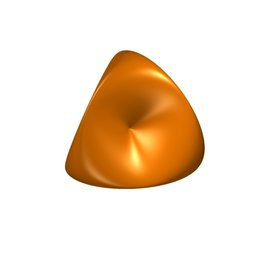
\includegraphics[height=1.4cm]{./../../common/images/kummer_0}
      \end{tabular}
      &
      \begin{tabular}{@{}c@{}}
        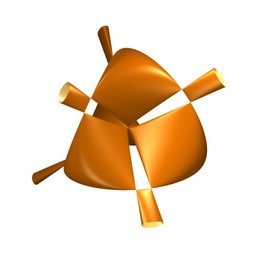
\includegraphics[height=1.4cm]{./../../common/images/kummer_1}
      \end{tabular}
      &
      \begin{tabular}{@{}c@{}}
        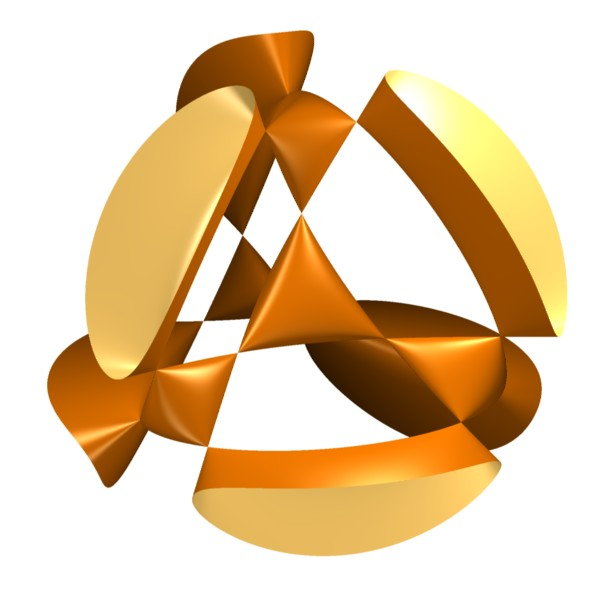
\includegraphics[height=1.4cm]{./../../common/images/kummer_2}
      \end{tabular}
      &
      \begin{tabular}{@{}c@{}}
        
\includegraphics[height=1.4cm]{./../../common/images/kummer_3}
      \end{tabular}
    \end{tabular}
  \end{center}
  \vspace{-0.2cm}  
     Pentru anumite valori speciale ale parametrului, c\^{a}teva dintre singularit\u{a}\c{t}i pot coincide.
\end{surferPage}
